\documentclass[10pt]{article}
\usepackage[a4paper,top=6mm,bottom=6mm,left=6mm,right=6mm,
            headheight=0pt,headsep=0pt,footskip=0pt]{geometry}
\usepackage[T1]{fontenc}
\usepackage{amsmath}
\usepackage{amssymb}
\usepackage{array}
\usepackage{xcolor}
\usepackage{tikz}
\usetikzlibrary{arrows.meta,decorations.pathreplacing}

% ================================================================
% Inequalities flashcards.
%
% One card for each skill on the topic list, with a second card where
% a skill splits into different methods. Each card is written once,
% with \flashcard{<skill>}{<question>}{<answer>}, and \printflashcards
% lays them out twenty to a sheet, four across and five down: a page
% of questions followed by a page of answers.
%
% The answer page mirrors the columns, so that when the file is
% printed double-sided, flipping on the long edge, each answer lands
% on the back of its own question. The left and right margins are
% equal so that the cut lines meet on both sides of the paper. Both
% sides of a card carry its number, so a card can still be matched to
% its answer if the printer shifts the back by a millimetre or two.
%
% The answers use the wording of the Maths Revision topic list. A key
% fact from that sheet is set in bold with \key, and each card ends with
% the sheet's "Remember" line for its topic, set in bold purple with
% \remember to match the purple lines on the sheet.
%
% A card whose contents are too tall for it is drawn with a red frame
% and reported in the log as FLASHCARD OVERFLOW.
% ================================================================

\pagestyle{empty}
\setlength{\parindent}{0pt}
\setlength{\parskip}{0pt}
\setlength{\topskip}{0pt}

\newcommand{\fctopic}{Inequalities}
\newcommand{\fccode}{Ineq}

% ----------------------------------------------------------------
% Card layout
% ----------------------------------------------------------------
\newlength{\fcw}\setlength{\fcw}{0.25\textwidth}
\newlength{\fch}\setlength{\fch}{56mm}
\newlength{\fcpad}\setlength{\fcpad}{2mm}
\newlength{\fciw}\setlength{\fciw}{\dimexpr\fcw-2\fcpad\relax}
\newlength{\fcgap}\setlength{\fcgap}{1.2mm}
\newlength{\fcspare}
\newlength{\fcbodytop}
\newsavebox{\fcheadbox}
\newsavebox{\fcbodybox}

% \flashcard{<skill>}{<question>}{<answer>} stores one card.
\newcounter{flashcard}
\newcommand{\flashcard}[3]{%
  \stepcounter{flashcard}%
  \expandafter\gdef\csname fcskill\arabic{flashcard}\endcsname{#1}%
  \expandafter\gdef\csname fcquestion\arabic{flashcard}\endcsname{#2}%
  \expandafter\gdef\csname fcanswer\arabic{flashcard}\endcsname{#3}}

% The idea a pupil must know to answer this type of question.
\newcommand{\key}[1]{{\bfseries\boldmath #1}}
% The quick way to remember the key step, worded as on the revision sheet.
\definecolor{remember}{RGB}{112,48,160}
\newcommand{\remember}[1]{{\color{remember}\bfseries\boldmath Remember: #1}}
% A line of working, centred and in display style. Used in place of \[ \],
% which leaves an empty line above it when it follows a paragraph break.
\newcommand{\working}[1]{\par{\centering$\displaystyle #1$\par}}

\newcommand{\fcquestionstyle}{\normalsize\raggedright\setlength{\parskip}{4pt}}
\newcommand{\fcanswerstyle}{\footnotesize\raggedright\setlength{\parskip}{2pt}}

% The strip across the top of a card: the skill on the front, and the
% card number on both sides.
\newcommand{\fcnumber}[1]{\makebox[10mm][r]{\color{black!55}\fccode\ #1}}
\newcommand{\fchead}[2]{%
  \begin{minipage}{\fciw}
    \scriptsize\color{blue!50!black}%
    \if#2Q\parbox[t]{\dimexpr\fciw-10mm\relax}{\raggedright\bfseries\csname fcskill#1\endcsname}%
    \else\textbf{Answer}\fi
    \hfill\fcnumber{#1}\par
    \vspace{0.6mm}%
    {\color{blue!30}\hrule height 0.4pt}%
  \end{minipage}}

% \fccard{<number>}{Q or A} draws one side of one card. Questions sit in
% the middle of the space under the strip; answers start at the top.
\newcommand{\fccard}[2]{%
  \sbox{\fcheadbox}{\fchead{#1}{#2}}%
  \sbox{\fcbodybox}{\begin{minipage}{\fciw}%
      \if#2Q\fcquestionstyle\csname fcquestion#1\endcsname
      \else\fcanswerstyle\csname fcanswer#1\endcsname\fi
    \end{minipage}}%
  \setlength{\fcbodytop}{\dimexpr\fcpad+\ht\fcheadbox+\dp\fcheadbox+\fcgap\relax}%
  \setlength{\fcspare}{\dimexpr\fch-\fcpad-\fcbodytop-\ht\fcbodybox-\dp\fcbodybox\relax}%
  \ifdim\fcspare<0pt
    \typeout{FLASHCARD OVERFLOW: \fccode\space #1 #2 by \the\dimexpr-\fcspare\relax}%
    \def\fccut{red}%
  \else
    \typeout{FLASHCARD SPACE: \fccode\space #1 #2 has \the\fcspare\space spare}%
    \def\fccut{black!35}%
    \if#2Q\addtolength{\fcbodytop}{0.5\fcspare}\fi
  \fi
  \begin{tikzpicture}
    \useasboundingbox (0,0) rectangle (\fcw,-\fch);
    \draw[line width=0.3pt,color=\fccut] (0,0) rectangle (\fcw,-\fch);
    \node[anchor=north west,inner sep=0pt] at (\fcpad,-\fcpad) {\usebox{\fcheadbox}};
    \node[anchor=north west,inner sep=0pt] at (\fcpad,-\fcbodytop) {\usebox{\fcbodybox}};
  \end{tikzpicture}}

\newcommand{\fctitle}[2]{%
  \hbox to \textwidth{\footnotesize\vrule width 0pt height 2.6mm depth 0.9mm
    {\color{blue!50!black}\bfseries\fctopic\ flashcards}\quad
    {\color{black!60}Sheet #1 of \fcsheets: \if#2Q questions\else answers\fi}\hfil
    {\color{black!60}Print double-sided, flipping on the long edge.}}%
  \vspace{1mm}}

% \fcpage{<sheet>}{Q or A}. On the answer page the columns run right to
% left, so that each answer is printed on the back of its question.
\newcommand{\fcpage}[2]{%
  \fctitle{#1}{#2}%
  \foreach \fcrow in {1,...,5}{%
    \nointerlineskip
    \hbox{\foreach \fccol in {1,...,4}{%
      \edef\fcn{\the\numexpr(#1-1)*20+(\fcrow-1)*4+\if#2Q\fccol\else(5-\fccol)\fi\relax}%
      \ifnum\fcn>\value{flashcard}%
        \hbox to \fcw{\vrule width 0pt height \fch\hfil}%
      \else
        \fccard{\fcn}{#2}%
      \fi}}}%
  \newpage}

\newcommand{\printflashcards}{%
  \pgfmathtruncatemacro{\fcsheets}{(\the\value{flashcard}+19)/20}%
  \foreach \fcsheet in {1,...,\fcsheets}{\fcpage{\fcsheet}{Q}\fcpage{\fcsheet}{A}}}

% ----------------------------------------------------------------
% Diagrams
% ----------------------------------------------------------------
% An operation written under both sides of an inequality, between the
% lines of working, as in the equations resources.
\newcommand{\op}[1]{{\scriptstyle\color{black!55}#1}}

% \numline{<drawing>}: a number line from -3 to 5. The drawing is
% placed at height 4, above the line.
\newcommand{\numline}[1]{%
  \begin{tikzpicture}[x=4.4mm,y=1mm,font=\scriptsize]
    \draw[{Stealth[length=1.3mm]}-{Stealth[length=1.3mm]}] (-3.7,0) -- (5.7,0);
    \foreach \n in {-3,...,5}{\draw (\n,-1) -- (\n,1); \node[below] at (\n,-1) {$\n$};}
    #1
  \end{tikzpicture}}
\newcommand{\opencircle}[1]{\draw[thick,blue!60!black,fill=white] (#1,4) circle (1mm);}
\newcommand{\filledcircle}[1]{\fill[blue!60!black] (#1,4) circle (1mm);}

\begin{document}

% ================================================================
% Number lines
% ================================================================
\flashcard{Reading inequalities on number lines}
{Write down the inequality shown on the number line.

{\centering
\numline{\draw[very thick,blue!60!black] (-1,4) -- (3,4); \opencircle{-1} \filledcircle{3}}\par}}
{\key{Number lines: open circle for $<$ or $>$ (not included), filled circle for $\le$ or $\ge$ (included)}

Open circle at $-1$: $x>-1$\\
Filled circle at 3: $x\le3$
\working{-1<x\le3}

\remember{Open circle: not included.\ \ Filled circle: included.}}

\flashcard{Drawing inequalities on number lines}
{Show $x\ge-2$ on a number line.

{\centering\numline{}\par}}
{Filled circle at $-2$, because $\ge$ includes $-2$:

{\centering
\numline{\draw[very thick,blue!60!black,-{Stealth[length=1.6mm]}] (-2,4) -- (5.6,4); \filledcircle{-2}}\par}

The arrow points right: $x$ can be $-2$ or any number bigger than $-2$.

\remember{Open circle: not included.\ \ Filled circle: included.}}

% ================================================================
% Solving inequalities
% ================================================================
\flashcard{Solving inequalities}
{Solve
\working{3x-5<13}}
{\working{\begin{array}{r@{\;}c@{\;}l}
  3x-5 & < & 13\\
  \op{+5} & & \op{+5}\\
  3x & < & 18\\
  \op{\div3} & & \op{\div3}\\
  x & < & 6
\end{array}}
($x$ can be any number less than 6)

\remember{Solve it like an equation, but keep the sign.}}

\flashcard{Solving inequalities with the unknown on both sides}
{Solve
\working{7x+4\ge3x+24}}
{\working{\begin{array}{r@{\;}c@{\;}l}
  7x+4 & \ge & 3x+24\\
  \op{-3x} & & \op{-3x}\\
  4x+4 & \ge & 24\\
  \op{-4} & & \op{-4}\\
  4x & \ge & 20\\
  \op{\div4} & & \op{\div4}\\
  x & \ge & 5
\end{array}}

\remember{Take away the smaller $x$-term from both sides first.}}

\flashcard{Solving double inequalities}
{Solve
\working{-3<2x+1\le9}
List the integer values of $x$ that satisfy the inequality.}
{\working{\begin{array}{r@{\;}c@{\;}c@{\;}c@{\;}l}
  -3 & < & 2x+1 & \le & 9\\
  \op{-1} & & \op{-1} & & \op{-1}\\
  -4 & < & 2x & \le & 8\\
  \op{\div2} & & \op{\div2} & & \op{\div2}\\
  -2 & < & x & \le & 4
\end{array}}
Integers: $-1$, 0, 1, 2, 3, 4\\
($-2$ is not included, as the sign is $<$; 4 is included, as the sign is $\le$)

\remember{Whatever you do to one part, do to all three parts.}}

\flashcard{Constructing inequalities}
{Cinema tickets cost £8 each, and there is a £5 booking fee for each order. Mia has £50.

Write an inequality for the number of tickets, $t$, that Mia can buy, and solve it.}
{Total cost $=8t+5$. Mia can spend at most £50, so $\le$:
\working{\begin{array}{r@{\;}c@{\;}l}
  8t+5 & \le & 50\\
  \op{-5} & & \op{-5}\\
  8t & \le & 45\\
  \op{\div8} & & \op{\div8}\\
  t & \le & 5.625
\end{array}}
$t$ is a whole number, so at most 5 tickets.

\remember{At most $\le$,\ \ at least $\ge$,\ \ more than $>$,\ \ less than $<$.}}

% ================================================================
% Inequalities on graphs
% ================================================================
\flashcard{Showing inequalities on a graph}
{Show the region $y<2x-1$ on a set of axes.

State whether the line is solid or dashed.}
{\key{Graphs: dashed line for $<$ or $>$, solid line for $\le$ or $\ge$}

\begin{minipage}[c]{0.52\linewidth}\raggedright
Draw $y=2x-1$ dashed.\\
Test $(2,0)$: $0<2\times2-1$, so $0<3$ \checkmark\\
Shade the side containing $(2,0)$.
\end{minipage}\hfill
\begin{minipage}[c]{0.44\linewidth}\centering
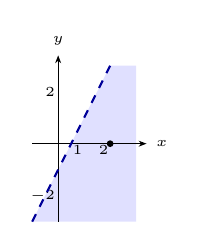
\begin{tikzpicture}[x=3.3mm,y=3.3mm,font=\tiny]
  \fill[blue!12] (-1,-3) -- (3,-3) -- (3,3) -- (2,3) -- cycle;
  \draw[black!15] (-1,-3) grid (3,3);
  \draw[-{Stealth[length=1mm]}] (-1,0) -- (3.4,0) node[right] {$x$};
  \draw[-{Stealth[length=1mm]}] (0,-3) -- (0,3.4) node[above] {$y$};
  \foreach \t in {1,2}{\node[below left,inner sep=0.5pt] at (\t,0) {$\t$};}
  \foreach \t in {-2,2}{\node[left,inner sep=1pt] at (0,\t) {$\t$};}
  \draw[thick,dashed,blue!60!black] (-1,-3) -- (2,3);
  \fill (2,0) circle (0.13);
\end{tikzpicture}
\end{minipage}

\remember{Dashed: not on it.\ \ Solid: on it.\ \ Test a point.}}

\flashcard{Reading regions on a graph}
{Write down the three inequalities that describe the shaded region R.

{\centering
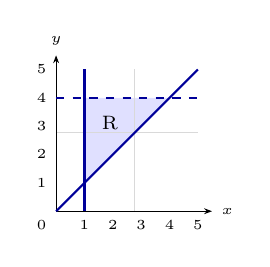
\begin{tikzpicture}[x=3.6mm,y=3.6mm,font=\tiny]
  \fill[blue!12] (1,1) -- (1,4) -- (4,4) -- cycle;
  \draw[black!15] (0,0) grid (5,5);
  \draw[-{Stealth[length=1mm]}] (0,0) -- (5.5,0) node[right] {$x$};
  \draw[-{Stealth[length=1mm]}] (0,0) -- (0,5.5) node[above] {$y$};
  \foreach \t in {1,...,5}{\node[below] at (\t,0) {$\t$}; \node[left] at (0,\t) {$\t$};}
  \node[below left] at (0,0) {$0$};
  \draw[thick,blue!60!black] (1,0) -- (1,5);
  \draw[thick,dashed,blue!60!black] (0,4) -- (5,4);
  \draw[thick,blue!60!black] (0,0) -- (5,5);
  \node[font=\scriptsize] at (1.9,3.1) {R};
\end{tikzpicture}\par}}
{\key{Graphs: dashed line for $<$ or $>$, solid line for $\le$ or $\ge$}

$x\ge1$: right of the solid line $x=1$\\
$y<4$: below the dashed line $y=4$\\
$y\ge x$: above the solid line $y=x$

Test a point in R, $(2,3)$:\\
$2\ge1$ \checkmark\quad $3<4$ \checkmark\quad $3\ge2$ \checkmark

\remember{Dashed: not on it.\ \ Solid: on it.\ \ Test a point.}}

% ================================================================
% Dividing by a negative number
% ================================================================
\flashcard{Dividing by a negative number}
{Solve
\working{5-3x>17}}
{\key{Multiplying or dividing both sides by a negative number flips the inequality sign}
\working{\begin{array}{r@{\;}c@{\;}l@{\quad}l}
  5-3x & > & 17\\
  \op{-5} & & \op{-5}\\
  -3x & > & 12\\
  \op{\div(-3)} & & \op{\div(-3)}\\
  x & < & -4 & \text{\scriptsize sign flipped}
\end{array}}
Check $x=-5$: $5-3\times(-5)=20>17$ \checkmark

\remember{Times or divide by a negative? Flip the sign!}}

\printflashcards

\end{document}
